
\documentclass{beamer}
\usepackage[latin1]{inputenc}
\usepackage{multirow}
\usetheme{Goettingen} %Warsaw
\usecolortheme{seagull}


\title[Experimental Design]{Experimental Design}
\subtitle{BCB 511: Applied Bioinformatics\\}
\author[Matt Settles]{Matt Settles}
\institute{University of Idaho}
\date{\today}


\begin{document}



%% Title page
\begin{frame}[plain]
  \titlepage
\end{frame}


%% Outline
\begin{frame}[plain] 
  \frametitle{Outline}
  \tableofcontents
\end{frame}

\section{Sample Preparation}

\begin{frame}
\begin{description}
\item[] In high throughput biological work (Microarrays, Sequencing, HT Genotyping, etc.), what may seem like small technical artifacts introduced during sample extraction/preparation can lead to large changes, or bias, in the data.
\item[]
\item[] Not to say this doesn't occur with smaller scale analysis such as Sanger sequencing or qRT-PCR, but they do become more apparent and may cause significant issues during analysis.
\end{description}
\end{frame}


\begin{frame}
 \frametitle{Sample Suggestions}
\begin{itemize}
\item Prepare more samples then you are going to need, i.e. expect some will be of poor quality, or fail.
\item Preparation stages should occur across all samples at the same time (or as close as possible) and by the same person
\item Spend time practicing a new technique to produce the highest quality product you can
\item Quality and quantity should be established using Fragment analysis traces (pseudo-gel images).
\item DNA/RNA should not be degraded,
\item BE CONSISTENT ACROSS ALL SAMPLES
\end{itemize}

\end{frame}

\section{Sequencing Needs}
\begin{frame}
\frametitle{Sequencing Depth}
\textbf{ The first and most basic question is how many base pairs of sequence data will I get}\\
Factors to consider are:
\begin{enumerate}
\item Number of reads being sequenced
\item Read length (if paired consider then as individuals)
\item Number of samples being sequenced
\item Expected percentage of usable data
\end{enumerate}

\begin{equation*}
bpPerSample = \frac{readLength*readCount}{sampleCount} * 0.8
\end{equation*}

\begin{alert}
The number of reads and read length data are best obtained from the manufacturer's website (search for specifications)  and always use the lower end of the estimate.
\end{alert}
\end{frame}


\begin{frame}
\frametitle{Coverage}
\textbf{Once you have the number of base pairs per sample you can then determine expected coverage}\\
Factors to consider are:
\begin{enumerate}
\item Length of the genome (in bp)
\item Any extra-genomic sequence, or contamination
\end{enumerate}

\begin{equation*}
expectedCoverage = \frac{bpPerSample}{totalGenomicContent}
\end{equation*}

\begin{alert}
Coverage is counted differently for "Counting" based experiments (RNAseq, amplicons) where an expected reads per sample is more suitable.
\end{alert}
\end{frame}

\begin{frame}
\frametitle{Read length and assembly}
\textbf{Read length matters}

\begin{figure}[htbp]
\begin{center}
   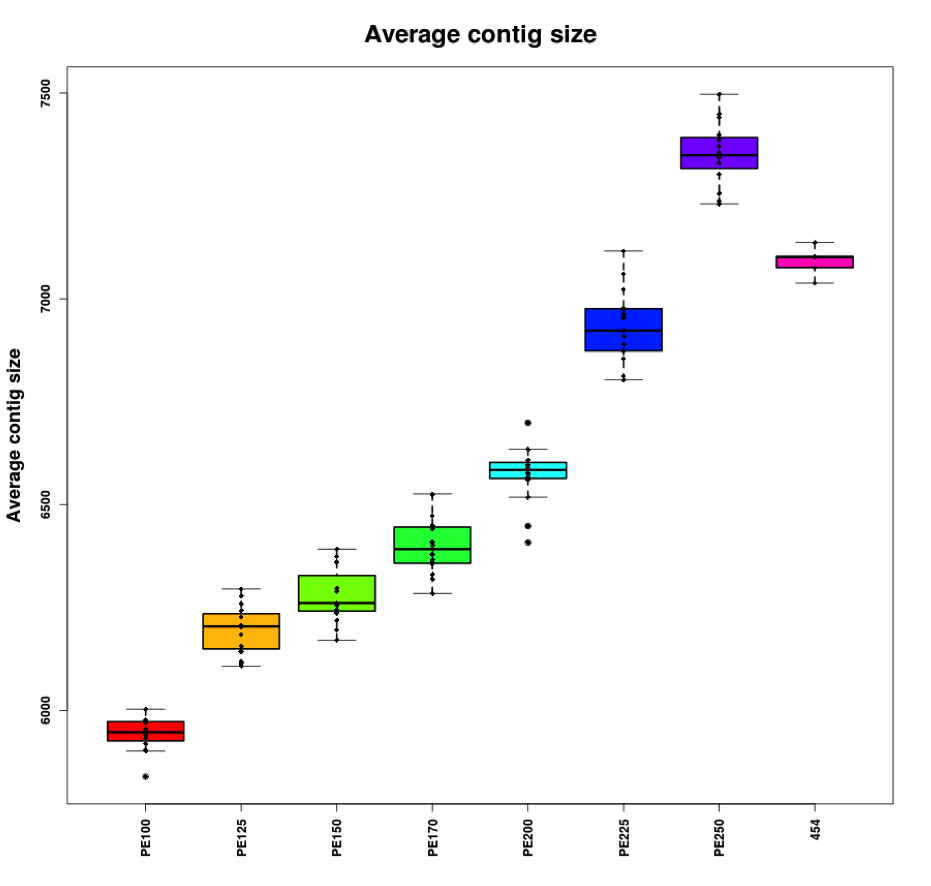
\includegraphics[scale=0.5]{assembly.png}
\end{center}
\end{figure}

\end{frame}

\begin{frame}
\frametitle{Coverage and mapping}
\textbf{Coverage in Variant calling matters}

\begin{figure}[htbp]
\begin{center}
   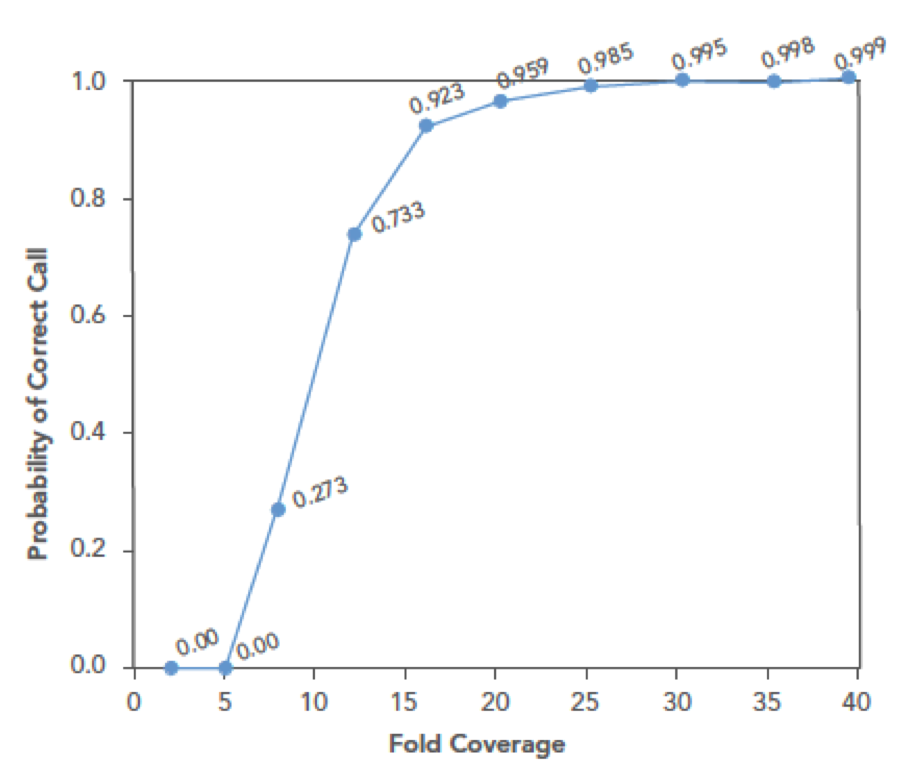
\includegraphics[scale=0.5]{mapping.png}
\end{center}
\end{figure}
\begin{alert}
Further, read length contributes to uniqueness of mapping
\end{alert}
\end{frame}

\begin{frame}
\frametitle{Metagenomics Coverage}
\textbf{First determine the dilution factor of the rarest species you want to sequence completely. For example if you wish to assemble a species that is present at 1 percent of the community, then your dilution factor is 1 in 100.}
\begin{equation*}
bpNeeded = \frac{DilutionFactor*AverageGenomeSize*Cov)}{0.8}
\end{equation*}
\begin{enumerate}
\item Average microbial genome size estimates\\ $2.5x10^6$ lower bound to $5.0x10^6$ mean estimate 
\item Coverage, 30x for Illumina
\end{enumerate}
\begin{alert}
Also consider the expected percentage of "contamination" in your calculation
\end{alert}
\end{frame}

\begin{frame}
\frametitle{RNAseq Coverages}
\textbf{Characterization of transcripts or Differential Gene Expression}

\begin{enumerate}
\item Read length needed depends on likelihood of mapping uniqueness, but generally longer is better and paired-end is better than single-end. 
\item Interest in measuring genes expressed at low levels
\item The fold change you want to be able to detect
\end{enumerate}

\begin{alert}
Uses the same equation as metagenomics (typical average gene sizes is 1500bp), average coverage should be greater
\end{alert}
\end{frame}




\section{Library Preparation}
\begin{frame}
 \frametitle{Library Preparation types}
 \begin{itemize}
 \item Shotgun - randomly fragmented DNA (100bp - 1kb) 
 \item RNA - Random nanomers or 3' bias (stranded or unstranded)
 \item Amplicons
 \item Selected (Capture, RADseq, etc.)
 \item Paired end / Mate pair
 \item Synthetic Long Reads
 \end{itemize}
\end{frame} 


\section{Sequence Data}
\begin{frame}
  \frametitle{fasta,qual and fastq files}
  \begin{itemize}
  \item fasta files\\%
  $>$sequence1\\
  ACCCATGATTTGCGA
  \item qual files\\%
  $>$sequence1\\
  40 40 39 39 40 39 40 40 40 40 20 20 36 39 39
  \item fastq files\\%
  $@$sequence1\\
  ACCCATGATTTGCGA\\
  $+$\\
  IIHHIHIIII55EHH
  \end{itemize}
\end{frame}

\begin{frame}
  \frametitle{phred scores}
$Q = -10log_{10}P$
\begin{center}
\begin{tabular}{|l|l|l|}
\hline
Phred & Probability &	Base call \\
Quality Score	& of incorrect  & accuracy \\
 & base call & \\
\hline
10	&	1 in 10	&	$90\%$\\
20	&	1 in 100 &	$99\%$\\
30	&	1 in 1000	&	$99.9\%$\\
40	&	1 in 10000	&	$99.99\%$\\
\hline
\end{tabular}
\end{center}
\end{frame}
% fasta
% qual
% fastq
%% quality scores
\begin{frame}
  \frametitle{phred score conversion}
$Q_{sanger} = -10log_{10}P$ - based on probability (aka phred)
\\

$Q_{solexa} = -10log_{10}\frac{P}{1-P}$ - based on odds
\begin{center}
\begin{tabular}{ l l l }
S - Sanger        &Phred+33,  &raw reads typically (0, 40) \\
X - Solexa        &Solexa+64, &raw reads typically (-5, 40) \\
I - Illumina 1.3+ &Phred+64,  &raw reads typically (0, 40) \\
J - Illumina 1.5+ &Phred+64,  &raw reads typically (3, 40) \\
L - Illumina 1.8+ &Phred+33,  &raw reads typically (0, 41) \\
\end{tabular}
\end{center}
\end{frame} 




\end{document}

